
\section{Fundamentação Teórica}\label{sec:fundamentacao}

SOC é um estilo arquitetural cujo objetivo é prover baixo acoplamento por meio
da interação entre agentes de software, chamados de serviços
\cite{he2003service}. A chave para que a solução baseada em SOC tenha
custo-benefício favorável é o reuso, o qual somente é possível se os serviços
possuírem interfaces ubíquas, com semânticas genéricas e disponíveis para seus
consumidores. Usualmente, a comunicação com os serviços, e entre eles, é feita
por meio da troca de mensagens com uso de \textit{servi\c cos web}, que seguem
padrões abertos de comunicação e que atuam sobre o protocolo HTTP. SOAP e
REST~\cite{fielding2000fielding} s\~{a}o as tecnologias mais usadas para
implementa\c c\~{a}o de servi\c cos web, sendo que REST tem ganhado mais
relevância nos \'{u}ltimos anos.

Entre os oito princípios para desenvolvimento SOA descritos
em~\cite{erl2008soa}, e\-xis\-te um especial interesse no \emph{contrato
padronizado} (\textit{Standardized Service Contract}), o qual sugere que
serviços de um mesmo inventário devem seguir os mesmos padrões de \textit{design}, de
modo a favorecer o reuso e a composição. Esse princípio prega a abordagem
\textit{Contract First}, em que a concepção do serviço parte da especificação do
contrato e não com a geração do contrato a partir código. \'{E} importante
destacar que n\~{a}o existe um padr\~{a}o para especificar contratos em REST, o
que motivou o desenho da \neoidl~\cite{bonifacio2015neoidl}, uma linguagem
espec\'{i}fica do dom\'{i}nio para especificação de contratos REST e que,
dife\-rente das linguagens existentes, prov\^{e} recursos de modularidade e
herança de tipos de dados customizados. Utilizando uma abordagem transformacional, a
\neoidl{} oferece suporte ferramental que gera c\'{o}digo fonte para diferentes
linguagens e plataformas REST, a partir de um conjunto de módulos \neoidl{} onde
são especificados os tipos de dados e os serviços.

A Figura \ref{lst:modulobasiconeo} apresenta um exemplo de módulo \neoidl{}
com a defini\c c\~{a}o de um tipo de dado \texttt{ItemDoCatalogo} e duas
opera\c c\~{o}es (chamadas de capacidades na terminologia REST):
\texttt{atualizarItem} (opera\c c\~{a}o do tipo POST associada ao
\emph{endpoint} \texttt{catalogo}) e \texttt{pesquisarItem} (opera\c c\~{a}o do
tipo GET, do mesmo \emph{endpoint}).


\begin{figure}[htb]
\begin{scriptsize}
\lstinputlisting[language=NeoIDL,firstnumber=1]{modulobasico.neo}
\end{scriptsize}
\caption{Exemplo de um módulo escrito em \neoidl}
\label{lst:modulobasiconeo}
\end{figure}


Conforme mencionado, o suporte ferramental da \neoidl{} processa um conjunto de
módulos escritos na linguagem \neoidl{}, gerando o código com a estrutura para
implementação dos serviços descritos.
A versão atual do ambiente \neoidl{} suporta geração de códigos em Java e Python
para as plataformas \emph{neoCortex}\footnote{propriet\'{a}ria do Ex\'{e}rcito
Brasileiro} e \emph{Twisted}. Entretanto, esse ambiente é extensível por meio
da implementação de novos plugins~\cite{bonifacio2015neoidl}.


%% \begin{figure}[ht] \centering
%% 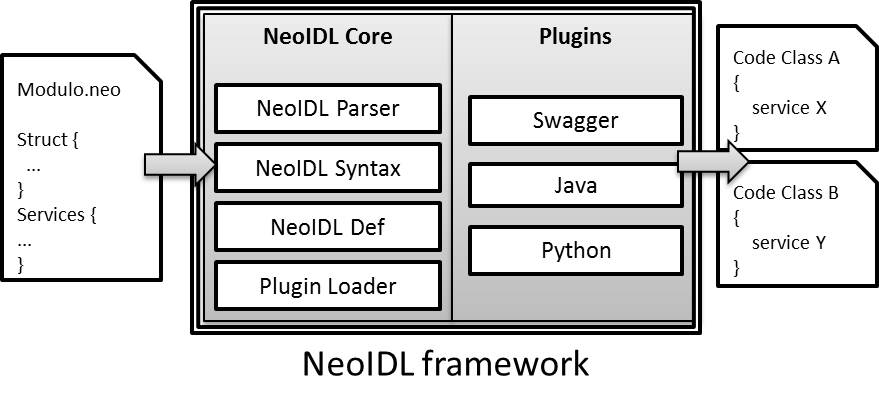
\includegraphics[width=.5\textwidth]{NeoIDLFrameworkArchtecture.jpg}
%% \caption{Entradas (lado esquerdo) e saídas (lado direito) do \textit{framework}
%% \neoidl}
%% \label{fig:NeoFrameArch}
%% \end{figure}

\emph{Limita\c c\~{a}o da \neoidl}. Atualmente a \neoidl{} permite apenas a
especifica\c c\~{a}o de \emph{weak contracts}, o que n\~{a}o permite estabelecer
obriga\c c\~{o}es entre fornecedores e clientes de servi\c cos. Esse tipo de
obriga\c c\~{a}o pode ser estabelecida com alguma t\'{e}cnica de
\emph{Design-by-contract}~\cite{meyer1992applying} (DBC) -- na qual o consumidor
e o fornecedor de servi\c cos firmam entre si um conjunto de garantias. Em um
contexto mais simples, de um lado o consumidor deve garantir que, antes da
chamada a um servi\c co (ou um m\'{e}todo de uma classe), os parâmetros de
entrada devem ser respeitados (essas garantias s\~{a}o denominadas 
pré-condições). Do outro lado, o fornecedor deve garantir que, uma vez
respeitadas as pré-condições, as propriedades relacionadas ao sucesso da
execução (pós-condições) s\~{a}o preservadas. DBC tem o objetivo de aumentar a
robustez do sistema e tem na linguagem Eiffel \cite{meyer1991eiffel} um de seus
precursores. Segundo Eiffel Software\footnote{Building bug-free O-O software: An
introduction to Design by Contract(TM).
https://archive.eiffel.com/doc/manuals/technology/contract/}, o uso de DBC na concepção de sistemas é uma abordagem sistemática que tende a reduzir a quantidade de erros observados nos sistemas.
Mais recentemente, algumas t\'{e}cnicas de \emph{design-by-contract} foram
especificadas e implementadas para outras linguagens de programa\c c\~{a}o, como
JML para a linguagem Java~\cite{leavens} e \texttt{Spec\#} para a linguagem
\texttt{C\#} (e demais linguagens da plataforma .NET)~\cite{barnett2005spec}.

% \subsection{NeoIDL}

